\section{Part 3}
    \subsection{Question}
    The weights of mature dogs of a certain breed approximately follow a normal distribution. Five dogs selected at random weighed 66, 63, 64, 62 and 65 pounds. A kennel club claims that the average weight for this breed is 60 pounds. Using the 0.05 level of significance, do we have reason to doubt this claim?

    \subsection{Answer}
    The null hypothesis, $H_{0}$, claims the mean weight of the breed is 60 pounds, while the alternative hypothesis, $H_{a}$, says otherwise.

        \[ H_{0}: \mu = 60 \ vs \ H_{a}: \mu \neq 60 \]

    Since the population standard deviation is unknown, and the sample was $n < 30$, the t-score was calculated as follows:

    The sample mean and standard deviation were calculated:
\begin{lstlisting}
    weights <- c(66, 63, 64, 62, 65)
    X <- mean(weights)
    s <- sd(weights)
\end{lstlisting}

        \[ t=\frac{\overline{X}-\mu}{\sfrac{s}{\sqrt{n}}}, \ df=4 \]\\
    \[ =\frac{64.0-60.0}{\sfrac{1.6}{\sqrt{5}}} \]
    \[ =t=5.6569, \ P(t)=-2.1318 \]


    The following snippet was used to generate the Z-value and its probability:
\begin{lstlisting}
    X <- 73.2
    mu <- 72.4
    sigma <- 2.1
    n <- 35

    z <- (X - mu)/(sigma/sqrt(n))
    print(z)  # print the Z-score
    print(pnorm(z))  # print the probability
\end{lstlisting}

    The test statistic was computed to be:

        \begin{align*}
            \because t_{0.025,4}=-2.7764 < 5.6569\\
        \end{align*}

    The p-value was computed with the following snippet:
\begin{lstlisting}
    pScore <- 2 * (1 - pt(score, df=n-1))
    # 0.004812
\end{lstlisting}

    Since $t_{\alpha, df} < t$ and the p-score was under 0.05, the null hypothesis is rejected.

    The box plot and normal probability plot were generated:

        \begin{figure}[ht]
            \begin{center}
                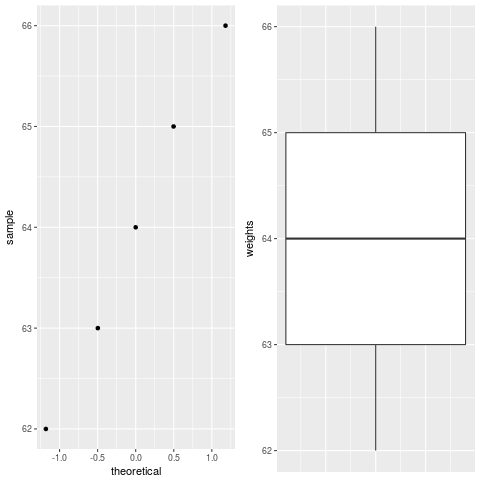
\includegraphics[width=0.5\textwidth]{figures/part3.png}
                \caption{Normal Probability Plot and Box Plot of the Distribution} \label{fig:part3}
            \end{center}
        \end{figure}
